% \documentclass{article}
\documentclass[a4paper,12pt]{article}
% \usepackage[T2A]{fontenc}
\usepackage{lmodern}
\usepackage[utf8]{inputenc}
\usepackage[T1]{fontenc}
\usepackage[english]{babel}
\usepackage[usenames,dvipsnames]{xcolor}
\usepackage{xspace}
\usepackage{mathrsfs}
\usepackage{graphicx}

\pagestyle{plain}
\usepackage[
  left=0.50in,
  right=0.50in,
  top=0.8in,
  bottom=0.7in,
  headheight=0.8in]{geometry}
\pagenumbering{gobble}

\setlength{\parskip}{0.15cm}

\usepackage{indentfirst}

\usepackage{hyperref}
\hypersetup{
  colorlinks,
  citecolor=black,
  filecolor=black,
  linkcolor=blue,
  urlcolor=blue
}

\usepackage{paralist}
\usepackage{cancel}
\usepackage{textcomp}
\usepackage{gensymb}
\usepackage{mdframed}
\usepackage{lastpage}
\usepackage{microtype}
\usepackage[super]{cite}
\usepackage{fancyhdr}
\pagestyle{fancy}


\newcommand\Section[2]{
  \newpage % new page
  \stepcounter{section}
  \bigskip
  \phantomsection
  \addcontentsline{toc}{section}{\arabic{section}. #1}
  \begin{center}
    {\huge \bf \arabic{section}. #1}\\
  \end{center}
  \bigskip
  \gdef\SectionName{#1}
  \gdef\AuthorName{#2}

  \lhead{\ShortCourseName}
  \chead{}
  \rhead{\SectionName}

  \cfoot{
%    \topskip0pt\vspace*{\fill}
    \thepage~from~\pageref*{LastPage}
%    \vspace*{\fill}
  }

  \renewcommand{\headrulewidth}{0.15 mm}

  \ifx\LaconicFooter\undefined
  \lfoot{
%    \topskip0pt\vspace*{\fill}
    Chapter \texttt{\#\arabic{section}}
%    \vspace*{\fill}
  }
  \rfoot{
%    \topskip0pt\vspace*{\fill}
    Author: \AuthorName
%    \vspace*{\fill}
  }
  \renewcommand{\footrulewidth}{0.15 mm}
  \fi
}



\newcommand\Subsection[1]{
  \subsection{#1}
}

\newcommand\Subsubsection[1]{
  \subsubsection{#1}
}

\newcommand\slashnl{~\\*[-26pt]}
\newcommand\slashn{~\\*[-22pt]}
\newcommand\slashns{~\\*[-18pt]}
\newcommand\slashnss{~\\*[-14pt]}
\newcommand\slashnsss{~\\*[-10pt]}

\newcommand{\makegood}{
  \ifx\ShortCourseName\undefined
  \gdef\ShortCourseName{\CourseName}
  \fi


  \ifx\NoTitlePage\undefined

  \ifx\CustomTitle\undefined
    \title{\CourseName}
    \maketitle
  \else
    \pagestyle{empty}
    \CustomTitle
  \fi
  \tableofcontents
  \pagebreak
  \fi

  \pagestyle{fancy}
  \pagenumbering{arabic}
  \setcounter{page}{1}

  \lhead{\ShortCourseName}

  \ifdefined\ENABLEDMATH
  \renewcommand\proofname{\em\textbf{Proof}}
  \else
  \fi
}


\newcommand{\TODO}[1][]{
  \vspace{0.2em}
  \textbf{{\bf\color{red} TODO:} #1}
  \vspace{0.2em}
}


\newcommand\enablemath{
  \usepackage{amsmath,amsthm,amssymb,mathtext}
  \usepackage{thmtools}
  \usepackage{tikz}

  \newcommand\R{\ensuremath{\mathbb{R}}\xspace}
  \newcommand\Q{\ensuremath{\mathbb{Q}}\xspace}
  \newcommand\N{\ensuremath{\mathbb{N}}\xspace}
  \newcommand\Z{\ensuremath{\mathbb{Z}}\xspace}
  \newcommand\CC{\ensuremath{\mathbb{C}}\xspace}

  \DeclareRobustCommand{\divby}{%
    \mathrel{\vbox{\baselineskip.65ex\lineskiplimit0pt\hbox{.}\hbox{.}\hbox{.}}}%
  }
  \newcommand\notmid{\centernot\mid}

  \let\Im\relax
  \let\Re\relax
  \DeclareMathOperator\Im{Im}
  \DeclareMathOperator\Re{Re}
  \DeclareMathOperator\res{res}

  \DeclareMathOperator*{\lcm}{lcm}
  \newcommand\vphi{\varphi}

  \usepackage{
    nameref,
    hyperref,
    cleveref}

  \ifx\ThmSpacing\undefined
  \def\ThmSpacing{9pt}
  \fi

  \ifx\ThmNamespace\undefined
  \def\ThmNamespace{section}
  \fi

  \declaretheoremstyle[
    spaceabove=\ThmSpacing, spacebelow=\ThmSpacing,
    headfont=\slshape\bfseries,
    bodyfont=\normalfont,
    postheadspace=0.5em,
  ]{thmstyle_def}

  \declaretheoremstyle[
    spaceabove=\ThmSpacing, spacebelow=\ThmSpacing,
    postheadspace=0.5em,
  ]{thmstyle_thm}

  \declaretheoremstyle[
    spaceabove=\ThmSpacing, spacebelow=\ThmSpacing,
    headfont=\itshape\bfseries,
    notefont=\itshape\bfseries, notebraces={}{},
    bodyfont=\normalfont,
    postheadspace=0.5em,
  ]{thmstyle_cons}

  \declaretheoremstyle[
    spaceabove=\ThmSpacing, spacebelow=\ThmSpacing,
    headfont=\bfseries,
    notefont=\bfseries, notebraces={}{},
    bodyfont=\normalfont,
    postheadspace=0.5em,
  ]{thmstyle_examp}

  \declaretheoremstyle[
    spaceabove=\ThmSpacing, spacebelow=\ThmSpacing,
    headfont=\ttfamily\itshape,
    notefont=\ttfamily\itshape, notebraces={}{},
    bodyfont=\normalfont,
    postheadspace=0.5em,
  ]{thmstyle_remark}

  \declaretheorem[numberwithin=\ThmNamespace, name=Theorem, style=thmstyle_thm]{theorem}
  \declaretheorem[numberwithin=\ThmNamespace, name=Definition, style=thmstyle_def]{definition}
  \declaretheorem[sibling=theorem, name=statement, style=thmstyle_thm]{statement}
  \declaretheorem[numbered=no, name=Note, style=thmstyle_remark]{remark}
  \declaretheorem[numbered=no, name=Lemma, style=thmstyle_thm]{lemma}
  \declaretheorem[numbered=no, name=Implication, style=thmstyle_cons]{consequence}
  \declaretheorem[numbered=no, name=Example, style=thmstyle_examp]{example}
  \declaretheorem[numbered=no, name=Properties, style=thmstyle_cons]{properties}
  \declaretheorem[numbered=no, name=Properties, style=thmstyle_cons]{property}

  \newcommand\thmslashn{\slashn}

  % Examples:
  % \begin{theorem} theorem-statement \end{theorem}
  %
  % Use theorem name in a title:
  % \begin{definition}[My name] the definition \end{definition}
  %
  % Create a mark for later use of a link:
  % \begin{statement}\label{stm:identifier} the statement \end{statement}
  %
  % \begin{statement}\label{otherlabel}
  %   \hyperref[stm:identifier]{Theorem}.
  %   \ref{stm:identifier}
  %   \autoref{stm:identifier} ‘‘\nameref{stm:identifier}’’,
  % \end{statement}

  \newcommand\eps{\varepsilon}
  \renewcommand\le{\leqslant}
  \renewcommand\ge{\geqslant}
  \newcommand\empysetold{\emptyset}
  \renewcommand\emptyset{\varnothing}

  \newcommand\ENABLEDMATH{YES}
}

\newcommand\enablecode{
  \usepackage{listings}
  \lstset{
    belowcaptionskip=1\baselineskip,
    breaklines=true,
    frame=L,
    xleftmargin=\parindent,
    showstringspaces=false,
    basicstyle=\footnotesize\ttfamily,
    keywordstyle=\bfseries\color{blue},
    commentstyle=\itshape\color{Maroon},
    identifierstyle=\color{black},
    stringstyle=\color{orange},
    numbers=left
  }

  \lstdefinestyle{supercpp} {
    language=C++,
    deletekeywords={int, long, char, short, unsigned, signed,
      uint64\_t, int64\_t, uint32\_t, int32\_t, uint16\_t, int16\_t, uint8\_t, int8\_t,
      size\_t, ptrdiff\_t, \#include,\#define,\#if,\#ifdef,\#ifndef},
    classoffset=1,
    morekeywords={vector,stack,queue,set,map,unordered\_set,unordered\_map,deque,array,string,multiset,multimap,
      int, long, char, short, unsigned, signed,
      uint64\_t, int64\_t, uint32\_t, int32\_t, uint16\_t, int16\_t, uint8\_t, int8\_t,
      size\_t, ptrdiff\_t
    },
    keywordstyle=\bfseries\color{green!40!black},
    classoffset=0,
    classoffset=2,
    morekeywords={std},
    keywordstyle=\bfseries\color{ForestGreen},
    classoffset=0,
    more comment=[l][\bfseries\color{purple!99!black}]{\#}
  }
}
% \usepackage{tabularx}
% \usepackage{systeme}

\enablemath

\begin{document}
\gdef\CourseName{GDSC: Algorithms \& Data Structures}
\author{Sergey Kopelevich, Vladislav Artiukhov}
\makegood

\Section{Big-O Notations}{Vladislav Artiukhov}

\Subsection{Definitions of $O, o, \Omega, \omega, \Theta$}
\Subsection{Asymptotic types: linear, quadratic, polylog, exponential}

For now refer to \textbf{GDSC Competitive Programming Abstract (topics 1-5), Fall 2023}.

\Section{Basic data structures}{Vladislav Artiukhov}

\Subsection{Arrays, doubly linked list, singly linked list}
\Subsection{std::vector and how it works internally}
\Subsection{stack, queue, deque}
\Subsection{Keeping minimum for $O(1)$: min-stack, min-queue implementation}

For now refer to \textbf{GDSC Competitive Programming Abstract (topics 1-5), Fall 2023}.

% TODO: create files for already written topics and insert move contents here

\Section{Master Theorem}{Vladislav Artiukhov}
\Subsection{Master Theorem}

Algorithms that are written in a recursive manner oftentimes utilize \textit{divide-and-conquer} technique which implies devision of the task into smaller subtasks that are processed by further recusive calls of the algorithm; once the subtask is small enough it is considered as a base case and processed manually. Some examples include \textbf{Merge sort algorithm}, \textbf{Binary search tree traversal}, etc.

For such algorithms we need to define their asymptotics. \textbf{Master Theorem} is a generalized method that yields asymptotically tight bounds for divide and conquer algorithms [\href{https://en.wikipedia.org/wiki/Master_theorem_(analysis_of_algorithms)#Generic_form}{wiki}].

\begin{theorem}
    \textbf{Master Theorem}

    Consider the following recurrence relation: $T(n) = a \cdot T(\frac{n}{b}) + f(n)$ where $f(n) = n^c$ for constants $a > 0, b > 1, c \geq 0$; let $k = \log_{b}{n}$ be the recursion depth. Then the following holds:

    \begin{equation}
        \begin{cases}
            T(n) = \Theta(a^k) = \Theta(n^{\log_{b}{a}}), \quad a > b^c\\
            T(n) = \Theta(f(n)) = \Theta(n^c), \quad a < b^c\\
            T(n) = \Theta(k \cdot f(n)) = \Theta(n^c \cdot \log{n}), \quad a = b^c\\
        \end{cases}
    \end{equation}

\end{theorem}



\begin{proof}

    $$ T(n) = f(n) + a \cdot T(\frac{n}{b}) = f(n) + a f(\frac{n}{b}) + a^2 f(\frac{n}{b^2}) + ... + a^k f(\frac{n}{b^k}) \quad | \ f(n)=n^c$$
    $$ T(n) = n^c + a\cdot (\frac{n}{b})^c + a^2\cdot (\frac{n}{b^2})^c + ... + a^k\cdot (\frac{n}{b^k})^c $$
    $$ T(b) = n^c \cdot (1 + \frac{a}{b^c} + (\frac{a}{b^c})^2 + ... + (\frac{a}{b^c})^k) $$

    Let $q = \frac{a}{b^c}$ and $S(q) = 1 + q + ... + q^k$:

    1. If $q=1$: $S(q) = 1 + 1 + ... + 1 = k+1 = \log_{b}{n} + 1 \implies T(n) = \Theta(f(n) \cdot \log{n})$.

    2. If $q<1$: $S(q)$ is a geometric progression, thus it is equal to $S(q) = \frac{1-q^{k+1}}{1-q} = const = \Theta(1) \implies T(n) = \Theta(f(n))$.

    3. If $q>1$: $S(q) = q^k + \frac{q^k-1}{q-1} = \Theta(q^k) \implies T(n) = \Theta(a^k \cdot (\frac{n}{b^k})^c) = \Theta(a^k)$.

    \textbf{Note}: $f(n)$ could be $O(n^c)$; it does not violate the proof ($f(n) = O(n^c) = C \cdot n^c$).

\end{proof}


\Subsection{Generalized Master Theorem}

\begin{theorem}
    \textbf{Generalized Master Theorem}

    In the case of $f(n) = n^c \cdot \log_{d}{n}$ Master Theorem still holds:

    $T(n) = a \cdot T(\frac{n}{b}) + n^c \cdot \log_{d}{n}$, $a>0, \ b>1, \ c\geq 0, \ d \geq 0$.

    \begin{equation}
        \begin{cases}
            T(n) = \Theta(a^k) = \Theta(n^{\log_{b}{a}}), \quad a > b^c\\
            T(n) = \Theta(f(n)) = \Theta(n^c \cdot \log^{d}{n}), \quad a < b^c\\
            T(n) = \Theta(k \cdot f(n)) = \Theta(n^c \cdot \log^{d+1}{n}), \quad a = b^c\\
        \end{cases}
    \end{equation}

\end{theorem}


\Subsection{Algorithm for recurrence relations}

There are also recurrence relations with the following form:

$T(n) = a_0 \cdot T(n - p_0) + a_1 \cdot T(n - p_1) + ... + a_k \cdot T(n-p_k) \quad a_i, p_i > 0, \ \sum p_i > 1$

There exists an algorithm of how to find asymptotics for such relations:

\begin{theorem}
    \textbf{Algorithm for recurrence relations}

    Given $T(n)$ of the above form with the above constants, then the following holds:

    $T(n) = \Theta(\alpha^n)$, such that $\alpha > 1$ and it is the \textbf{only root} of the equation: $\alpha^n = a_0 \cdot \alpha^{n-p_0} + ... + a_k \cdot \alpha^{n-p_k}$

    % TODO: add proof

\end{theorem}


\begin{example}
    \textbf{Use of Master Theorem}

    1. $T(n) = 4 \cdot T(\frac{n}{2}) + 20 \cdot n^\frac{3}{2}$

    $a=4, \ b=2, \ c=\frac{3}{2}, \ f(n)=20\cdot n^\frac{3}{2} \implies a=4 > b^c=\sqrt{8} \implies T(n) = \Theta(n^{log_{b}{a}}) = \Theta(n^2)$.

    2. Merge sort algorithm recurrence relation: $T(n) = 2 \cdot T(\frac{n}{2}) + C\cdot n^1$

    $a=2, \ b=2, \ c=1 \implies a=4 = b^c=2^1 \implies T(n) = \Theta(n^1 \cdot \log{n})$

\end{example}


\begin{example}
    \textbf{Use of Algorithm for recurrence relations}

    1. $T(n) = T(n-1) + 6 \cdot T(n-2)$

    $T(n) = \Theta(\alpha)$, notice that $\alpha = 3$ satisfies the equation: $3^n = 3^{n-1} + 6 \cdot 3^{n-2}$.

    2. $T(n) = T(n-1) + T(n-2) + T(n-3)$

    $1 = \alpha^{-1} + \alpha^{-2} + \alpha^{-3} \implies \alpha \approx 1.839$

    % TODO: add Fibbonachi numbers

\end{example}

\Section{Amortized Analysis}{Vladislav Artiukhov}
\Subsection{Definition and general perception of the concept}

Remember that we were talking about \textbf{std::vector} we said that its \textbf{push\_back} operation works for an average of $\Theta(1)$. It was due to presence of 2 \textbf{distinct states}:

1. vector has enough capacity to fit the next pushed element.

2. vector does not have enough capacity and has to make itself twice bigger (i.e. reallocating a memory buffer of size $2\cdot N$).

There are definetely more complicated senarios where number of such \textit{interesting states} is much greater, thus we need a unified approach of how to define this average, or \textbf{amortized}, time for an operation.

\begin{definition}
    \textbf{The amortized analysis}

    The amortized analysis is an approach that allows to determine an average running time (time complexity) of operations $o_1$, $o_2$, ..., $o_k$ in a sequence $S$ over that sequence $S$.

\end{definition}

There are several methods that are referred to as amortized analysis (\href{https://en.wikipedia.org/wiki/Amortized_analysis}{wiki}). We are going to discuss \textbf{Potential method}.

\Subsection{Amortized analysis: Potential method}

\begin{definition}
    \textbf{Potential method}

    % TODO: use \varphi + use \mathbb instead of \mathbf, inf -> \infty

    Introduce a \textbf{potential function} called $\Phi: \mathbf{S} \to \mathbf{R_{0}^{+}}$ where $\mathbf{S}$ is a set of states of the considered data structure and $R_{0}^{+} = [0, +\inf)$, i.e. the potential function maps states of the data structure to some non-negavite values. As an important edge case for the initial state $S_{init}$: $\Phi(S_{init}) = 0$.

    Let $o_i$ be an individual operation within some sequence of operations named $Q$. Let $S_{i-1}$ be the state of the considered data structure before the execution of the operation $o_i$ and $S_{i}$ be the state after the execution of $o_i$. Let $\Phi$ be a chosen potential function, then the amortized time for an operation $o_i$ is defined as follows:

    $ T_{a}(o_i) = T_{r}(o_i) + \left (\Phi(S_{i}) - \Phi(S_{i-1}) \right ) $ where:

    1. $T_{a}(o)$ - amortized time of the operation.

    2. $T_{r}(o)$ - real/actual time spent on the operation.
\end{definition}

\begin{theorem}
    \textbf{Potential method yields an upper bound}

    The amortized time of a sequence of operations always yields an \textbf{upper bound} of the the real/actual time for the considered sequence of operations, i.e.:

    $\forall O = o_1, o_2, ..., o_n$ be a sequence of operations, define:

    1. $T_{a}(O) = \Sigma_{i=1}^{n} T_{a}(o_i)$ - amortized time of the sequence $O$

    2. $T_{r}(O) = \Sigma_{i=1}^{n} T_r(o_i)$ - real time of the sequence $O$

    Then: $T_r(O) \leq T_a(O)$

\end{theorem}

\begin{proof}

    As definition for $T_a(O)$ suggests:

    $$ T_{a}(O) = \Sigma_{i=1}^{n} (T_{r}(o_i) + \Phi(S_i) - \Phi(S_{i-1})) = T_{r}(O) + \Phi(S_n) - \Phi(S_0) $$
    $$ T_{a}(O) = T_{r}(O) + \underbrace{\Phi(S_n)}_{\cdot \geq 0} - \underbrace{\Phi(S_0)}_{\cdot = 0} \geq T_{r}(O) $$

\end{proof}

\underline{Note}: Generally speaking, $\Phi$ could be any function that satisfies the constraints but the idea is to find such $\Phi$ that would represent the closest upper bound of the real/actual time for the considered sequence of operations.

\begin{example}
    \textbf{Amortized analysis for std::vector::push\_back operation}

    1. Analyse push\_back operation that expands the vector:

    Let $\Phi = 2 \cdot s - N$ where the $s$ is the actual size of a vector and $N$ is its capacity. Remember that the expansion occurrs once $s == N$.

    Let's consider a push\_back operation that doubles the size of the vector:

    1. $T_{r} = s+1 = N+1$ - because we need to copy all the existing elements in a new buffer + place a new element; here $s=N$ because the extention could only happen once $s=N$.

    2. $\Phi_0 = 2\cdot s - N \geq 0$ - value of the potential function before the operation.

    3. $\Phi_1 = 2\cdot (s + 1) - 2N \geq 0$ - value of the potential function after the operation.

    Thus, we have:

    $T_a = T_r + \Phi_1 - \Phi_0 = N+1 + (2s + 2 - 2N - 2s + N) = N+1 + (2-N) = N-N+3 = \Theta(1)$.\newline


    2. Analyse push\_back operation that does not expand the vector:

    Notice that in this case $\Delta\Phi = \Phi_1 - \Phi_0 = const$ and $T_r = const$, thus $T_a = const = \Theta(1)$.\newline

    For more examples check the \href{https://en.wikipedia.org/wiki/Potential_method#Multi-Pop_Stack}{wiki} page.


\end{example}

\Section{Binary Search}{Vladislav Artiukhov}
\Subsection{Definition, use cases}

\Subsubsection{Simplest version}

Given a sorted array of size $n$. We need to find and element $x$ in this array for $O(\log{n})$:


\begin{lstlisting}[language=C++]
int find(int l, int r, int x) { // [l,r]
    // a is sorted in the ascending order
    while(l <= r) {
        int m = (l + r) / 2;
        if (a[m] == x) return m;
        else if (a[m] < x) l = m + 1;
        else r = m - 1;
    }
    return -1; // i.e., not found
}
\end{lstlisting}

The time complexity is indeed $O(\log{n})$ since on each iteration the $|r - l|$ decreases its value in a half ($|r - l| \to \frac{|r-l|}{2}$).

The problem of such an implementation is that if there are multiple occurrences of $x$ in the array, the algorithm will return \textbf{some index} in a range $[l_{ans}, \ r_{ans})$ where $\forall i=l_{ans}, ..., r_{ans}-1: \ a[i] == x$, although we would like to get either of both sides of the range, i.e. either $l_{ans}$ or $r_{ans}$.

\Subsubsection{Lower bound / Upper bound}

The above problem leads to the following implementations of the binary search algorithm that searches for the forementioned indicies:

1. $\min{i}: a_i \geq x$, i.e. $l_{ans}$:

\begin{lstlisting}[language=C++]
int lower_bound(int l, int r, int x) {
    while (r - l > 1) {
        int m = (l + r) / 2;
        if (a[m] < x) l = m; // Notice that we keep the invariant: a[l] < x
        else r = m; // => a[r] >= x
    }
    // (a[l] < m) && (a[r] >= m) => r is a minimum index
    return r;
}
\end{lstlisting}

2. $\min{i}: a_i > x$, i.e. $r_{ans}$:

\begin{lstlisting}[language=C++]
int upper_bound(int l, int r, int x) {
    while(r - l > 1) {
        int m = (l + r) / 2;
        if (a[m] > x) r = m;
        else l = m;
    }
    // Now a[r] > x => l is the last index for which a[l] <= x
    return r;
}
\end{lstlisting}

\begin{center}
    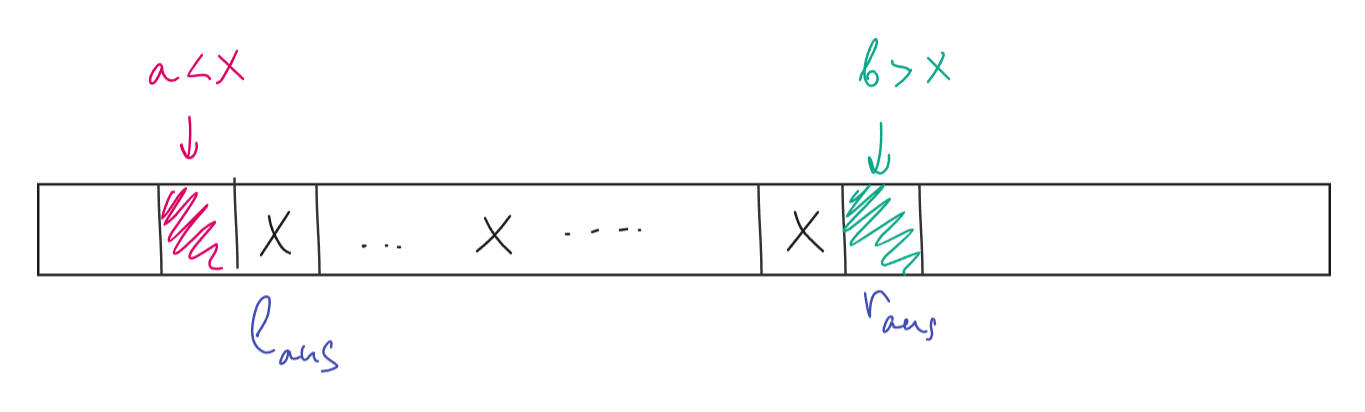
\includegraphics[scale=0.6]{./assets/08-binary-search/1.PNG}
\end{center}


\Subsubsection{STL implementation}

In C++ language we are already provided with the template functions that do the same thing:

\begin{lstlisting}[language=C++]
/* returns iterator (for int* it is a pointer) */
int i = std::lower_bound(a, a + n, x) - a;
int i = std::upper_bound(a, a + n, x) - a;

// For other containers (e.g., std::vector, std::set) that define begin()/end() operations use the following:
std::lower_bound(
    std::begin(container),
    std::end(container),
    element
) //  e.g., for std::vector<T> the return type is std::vector<T>::iterator, i.e. pointer to the element
\end{lstlisting}


\Subsection{Use of a predicate}

We could abstract the implementation even further via searching for a predicate. Predicate is such a function $f: S \to \{0, 1\}$. Then let's consider the predicate $f(i) = if (a_i < x) then 0 else 1$ - in this case the binary search will find such indicies $l$ and $r$ that satisfy the following:

1. $l + 1 = r$

2. $f(l) = 0$ (i.e. $a_l < x$)

3. $f(r) = 1$ (i.e. $a_r >= x$)

\begin{lstlisting}[language=C++]
int binary_search(int l, int r, int x) {
    while(r - l > 1) {
        int m = (l + r) / 2;
        if (f(m)) r = m; // invariant: a[r] >= x
        else l = m; // invariant a[l] < x
    }
    return r;
}

// If you want to parameterize predicate as well:
// #1: provide a 4th argument as a pointer to a function
// (see: https://www.cprogramming.com/tutorial/function-pointers.html)
int binary_search(int l, int r, int x, bool(*f)(int)) {
    ...
}

// #2: template parameter
template<typename /* or class */ Func>
int binary_search(int l, int r, int x, Func f) {
    ...
}
// possible call:
binary_search(l, r, x, []() { /* predicate impl */ });
\end{lstlisting}

\Subsection{Correctness}

You might already noticed that the functions (arrays are also akin functions, i.e. $a: \{0, 1, .., n-1\}: \mathbb{N} $) over which we apply the binary search algorithm are all monotonic functions, i.e. they comply to $x < y: \ f(x) < f(y)$ (strict monotonically increasing functions; the rest are alike).

\begin{lemma}
    \textit{The binary search algorithm over some range [x, y) is correct iff the considered function $f$ is monotonic over [x, y).}
\end{lemma}



\Subsection{Binary search for functions over $\mathbb{R}$}

It is possible to use the binary search with real numbers as well. Let's consider a problem of \textit{finding square root of} $x$:

\underline{\textbf{Problem statement}}: Given $x \in \mathbb{R}$. Find a value $y \in \mathbb{R}$ so that $y^2 == x$ (for us it is $|y^2 - x| < \varepsilon$):

\begin{lstlisting}[language=C++]
double my_sqrt(double x /* never use 'float' */) {
    double l = 0.0;
    double r = x + 1;

    const dobule EPS = 1e-9; // 10^(-9)

    while(r - l > EPS) {
        double m = (r + l) / 2;
        // Preserve invariant: l^2 <= x, r^2 > x
        if (m*m > x) r = m;
        else l = m;
    }

    return (l + r) / 2;
}
\end{lstlisting}

In the above notice: if $0 < y < 1$ then $y^2 < y$, and if $y \geq 1$ then $y^2 \geq 1$. Thus, for $0 < x < 1$ the corresponding $y$ is greater than $x$, i.e. we select $r = x + 1$.

\begin{example} \textbf{Root of a polynomial} $\mathbf{P(x)}$

    Given a polynomial $P(x)$ of \textbf{an odd degree}, i.e. $\deg{P} = 2k + 1$ with the coerfficient for $x^{2k+1}$ be equal to $1$. There exists a root $x_0 \in \mathbb{R}$, and we need to find it.

    \underline{\textbf{Solution}}:

    We could do that using binary search with any precision $\varepsilon$. First, we need to find points $l$ and $r$, such that: $P(l) < 0$ and $P(r) > 0$ (e.g., $l=-\infty, \ r=+\infty$ - \textbf{MAX\_INT} and \textbf{MIN\_INT} in C++):

    \begin{lstlisting}[language=C++]
    for (l = -1; P(l) >= 0; l *= 2);
    for (r = 1 ; P(r) <= 0; r *= 2);
    \end{lstlisting}

    And finally the root search:

    \begin{lstlisting}[language=C++]
        while (r - l > EPS) {
            double m = (l + r) / 2;
            if (P(m) < 0) l = m; // P(l) < 0
            else r = m; // P(r) >= 0
        }
        return (l + r) / 2;
    \end{lstlisting}

    Actually we need exactly $k := \frac{r-l}{\varepsilon}$ iterations, thus the while-loop could be changed by the for-loop.

\end{example}

\end{document}